\chapter{Sprint zéro}
\section*{Introduction}
Dans le chapitre précédent, nous avons évoqué le choix de la méthode Scrum. Maintenant nous passerons à la phase la plus importante de cette méthodologie, communément appelée « Sprint Zéro » qui permet de créer le squelette de base du projet afin que les futurs sprints puissent donner une valeur ajouter de manière efficace.
\section{Capture des besoins}
La phase de capture des besoins est la première phase formelle obligatoire dans le développement d’une application informatique puisque la capacité de persuasion d’un produit ne peut se réaliser parfaitement sans une spécification préalable élaborée des besoins et des exigences.
\subsection{Identification des acteurs}
Nous précédons par une détermination des acteurs. Un acteur est toute entité qui interagit avec notre système dans le but de réaliser une plus-value et qui a toujours le même comportement.\\
Notre application interagit avec les acteurs suivants :
\begin{itemize}
    \item \textbf{administrateur} : La personne responsable de la création des statistiques et des comptes clients.
    \item \textbf{administrateur} : : Cet acteur peut créer des Dashboards avec les statistiques déjà crées par un administrateur. 
\end{itemize}

\subsection{Besoins non fonctionnels}
Il s’agit d’un ensemble de règles à respecter lors du développement d'un projet pour s'assurer de la bonne utilisation de l'application. Nos besoins non fonctionnels se résumes principalement en :

\begin{itemize}
    \item l'ergonomie : \\
L’application doit être simple et facile à manipuler par l’utilisateur. Le passage entre les interfaces de l’application doit se faire dans des délais prompts. Une alerte prévient l’utilisateur, chaque fois qu’il commet une erreur d’utilisation.  
    \item la fiabilité : \\
Touche à l’aspect qualité des données et persistance des informations dans l’application ainsi que la vitesse de chargement des interfaces, elle doit aussi fonctionner d’une façon cohérente sans erreur.
    \item la sécurité : \\
Tous les accès aux différents espaces doivent être protégés par un mot de passe et un privilège d'accès. Ainsi, il faut s'assurer des cryptages des données au niveau de la base.
\end{itemize}

\subsection{Besoins fonctionnels}

Les besoins fonctionnels définissent le fonctionnement d’un système ou l’un de ses sous-systèmes, cela dépende aussi du type de logiciel, des utilisateurs finaux et du type de système dans lequel le logiciel est utilisé. Nous avons dégagé les principaux besoins fonctionnels de notre système qui se résume en :
\begin{itemize}
    \item authentification \\
    L’administrateur ou l’agent doivent s’authentifier avec un login et un mot de passe avant n’importe quelle interaction avec l’application.
    \item gestion des statistiques \\
    L’administrateur peut créer des statistiques de plusieurs types, il peut aussi les modifiées ou les supprimées ainsi que les partagé avec des utilisateurs ou des profils afin que ses derniers peuvent les utilisées pour construire un Dashboard.
    \item gestion de Dashboard \\
    L’agent peut créer des Dashboard avec les statistiques créer par l’administrateur, cet agent peut partager le Dashboard créer afin que d’autres utilisateurs peuvent le consulter.
    \item gestion des ressources \\
    Afin de créer des statistiques l’administrateur doit pouvoir utilisées des ressources.
    \item gestions des utilisateurs \\
    L’administrateur peut créer des comptes utilisateurs et leurs assigner à des profils.
\end{itemize}




\subsection{Diagramme des cas d'utilisations global}
La figure \ref{fig:ucgloab} représente le diagramme des cas d'utilisation global, qui modélise les fonctionnalités que doit assurer notre système.
\begin{figure}[htpb]
\centering
    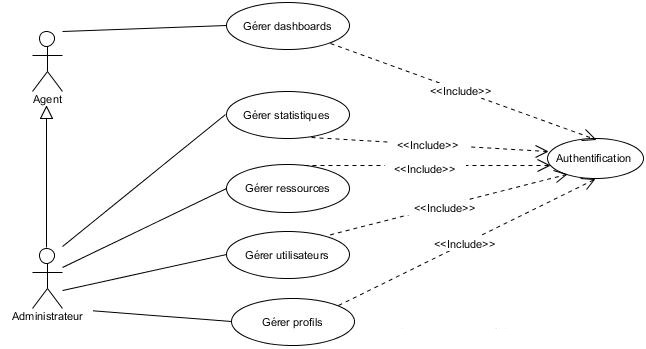
\includegraphics{Global}
    \caption{Diagramme de cas d'utilisations global}
    \label{fig:ucgloab}
\end{figure}

\section{\'Etude technique}
Cette section présente l’environnement matériel mis à la disposition du présent projet ainsi que l’environnement logiciel qui a permis à l'aboutissement de la mise en \oe uvre de l'application.
\subsection{Architecture matérielle}
Le choix de l’architecture d’une application est d’une importance primordiale et influencera sur les performances, l'évolutivité, les temps de développement, et bien sûr les coûts. De nos jours, une séparation des applications en différentes couches est requise, et nous parlons alors d’applications multi-niveaux ou multi-tiers (n-tiers), d’où l’architecture 3 tiers montré dans la figure \ref{fig:architecture} \cite{3tiers} ci-dessous, que nous avons choisi de l’utiliser pour réaliser notre projet.
\begin{figure}[htpb]
\centering
    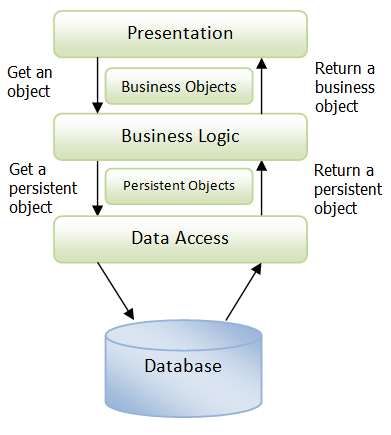
\includegraphics[scale=0.7]{3tiers}
    \caption{Architecture 3 tiers}
    \label{fig:architecture}
\end{figure}
\newpage
Les trois niveaux d'une architecture à trois niveaux sont les suivants :
\begin{itemize}
    \item couche de présentation : \\
    c'est le niveau le plus élevé de l'application. La couche de présentation fournit l'interface utilisateur de l'application. \\
     Dans notre cas le client est un navigateur Web.
    \item couche métier : \\
     c'est le logique métier, ce niveau est tiré du niveau de présentation. Il contrôle la fonctionnalité de l'application en effectuant un traitement détaillé. \\
     Dans notre cas nous avons utilisé le serveur d’application Java EE JBOSS EAP 7. Étant écrit en Java, JBOSS EAP 7 peut être utilisé sur tout système d’exploitation fournissant une machine virtuelle Java (JVM).
    \item couche d'accès aux données : \\
    c'est niveau où les informations sont stockées et récupérées. Les données de ce niveau sont indépendantes des serveurs d'applications ou de la logique métier. \\
    Nous avons, dans notre cas, utilisé le SGBDR (Système de Gestion de Base de Données Relationnelles), Oracle 11g.
\end{itemize}

\subsection{Architecture applicative}
Une bonne architecture applicative est une architecture qui permet de maintenir facilement l'application. Dans ce cadre notre choix s’est orienté vers l’architecture Modèle-Vue-Contrôleur (MVC), qui permet la structuration d'une application par la séparation en couches. MVC sépare les aspects traitement, données et présentation, et définit les interactions entre ces trois aspects. La figure \ref{fig:mvc} \cite{mvc} présente donne un aperçu de l’architecture obtenu.

\begin{figure}[htpb]
\centering
    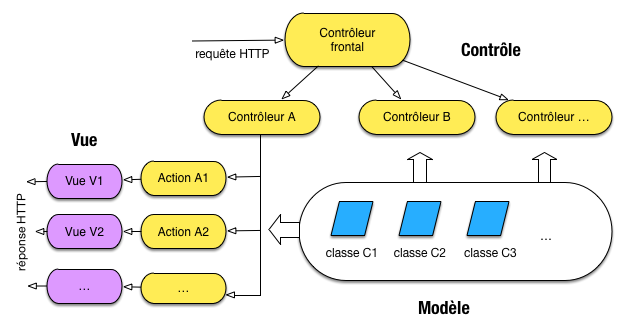
\includegraphics[scale=0.7]{mvc}
    \caption{MVC}
    \label{fig:mvc}
\end{figure}
Les trois couches qui constitue MVC sont :
\begin{itemize}
    \item le modèle : \\
    correspond à toutes les logiques liées aux données avec lesquelles l'utilisateur interagit. Cela peut représenter soit les données qui sont transférées entre les composants vue et contrôleur, soit toute autre donnée liée à la logique métier.
    \item la vue : \\
    est responsable de l'interface, ce qui recouvre essentiellement dans notre cas les fragments HTML qui sont assemblés pour constituer les pages de l'application. La vue est également responsable de la mise en forme des données.
    \item le contrôleur : \\
    permet de récupérer les données utilisateurs, de les filtrer et de les contrôler, de déclencher le traitement approprié (via le modèle), et finalement de déléguer la production du document de sortie à la vue.
\end{itemize}

\subsection{Environnement logiciel}
Le choix des logiciels à utiliser est aussi important que le choix architectural. Il s’agit d’un ensemble de logiciels qui seront utilisés tout au long du cycle de vie du projet, par conséquent
leur performance, leur disponibilité et leur stabilité influencent directement la qualité du produit réalisé. Étant donné que tout choix doit être étudié et justifié, nous avons dans notre cas utilisé
des logiciels proposés par la société, soit par obligation de compatibilité, soit par préférence.
\subsubsection{Outil de conception}
\paragraph{Langage de modélisation UML 2  \\}
UML est l'acronyme de Unified Modeling Language est un langage de modélisation fondé sur les concepts orientés objets. Il sert à modéliser les phénomènes de l'activité d'une entreprise sans tenir compte des techniques d'implémentation. UML utilise une
notation graphique fondée sur des diagrammes. UML n'impose pas une démarche particulière pour l'analyse d'un système mais préconise d'adopter une démarche ayant les caractéristiques suivantes :
\begin{itemize}
    \item Itérative et incrémentale
    \item Centrée sur l'architecture logicielle
    \item Guidée par le besoin des utilisateurs du système  
\end{itemize}

\paragraph{Visual Paradigm For UML \\}
Visual Paradigm For UML : permet la création des diagrammes UML et des modèles qui en sont à l'origine.\\
Ces diagrammes peuvent générer du code dans un langage de programmation déterminé. Visual Paradigm
For UML propose la création de plusieurs autres type de diagrammes, il peut modélisé les diagrammes de base
de données et générer du code SQL.

\subsubsection{Outil de développement}
\paragraph{Oracle 11g \\}
Oracle Database est un système de gestion de base de données relationnelle (SGBDR), édité par la société Oracle Corporation.
Oracle 11g comprent : 
\begin{itemize}
    \item la base de données (les fichiers physiques sur le disque),
    \item l'instance Oracle qui comprend la structure de la mémoire et les processus d'arrière plan et ceux du serveur,
    \item Oracle Net, la couche logicielle permettant aux applications clientes et à la base de données de communiquer sur un réseau.
\end{itemize}

\paragraph{JBoss EAP \\}
JBoss EAP est basé sur la version le serveur d'application WildFly,
il fournit des options préconfigurées pour les fonctionnalités telles que la messagerie et la mise en cache distribuée. Il permet également aux utilisateurs d'écrire, de déployer et d'exécuter des applications à l'aide des différentes API et services fournis par JBoss EAP.\\
JBoss EAP comprend une structure modulaire qui permet l'activation de service uniquement lorsque cela est requis, ce qui améliore la vitesse de démarrage. La console de gestion basée sur le Web et l'interface de ligne de commande de gestion (CLI) rendent l'édition des fichiers de configuration XML inutiles et ajoutent la possibilité de script et d'automatiser les tâches.JBoss EAP comprend aussi des API et des frameworks de développement pour développer rapidement des applications Java EE sécurisées et évolutives.

\subsection{Technologies utilisées}
\subsubsection{Plate-formes}
\paragraph{Java EE \\}
Java EE ou Java Platform, Enterprise Edition est une plate-forme fortement orientée serveur pour le développement et l'exécution d'applications distribuées. Elle est composée de deux parties essentielles :
\begin{itemize}
    \item un ensemble de spécifications pour une infrastructure dans laquelle s'exécutent les composants écrits en Java : un tel environnement se nomme serveur d'applications,
    \item 	un ensemble d'API qui peut être obtenues et utilisées séparément. Pour être utilisées, certaines nécessitent une implémentation de la part d'un fournisseur tiers,
\end{itemize}
L'utilisation de Java EE pour développer et exécuter une application offre plusieurs avantages :
\begin{itemize}
    \item une architecture d'applications basée sur les composants qui permet un découpage de l'application et donc une séparation des rôles lors du développement,
    \item La possibilité de s'interfacer avec le système d'information existant grâce à de nombreuses API : JDBC, JNDI, JMS, JCA ...,
    \item 	la possibilité de choisir les outils de développement et le ou les serveurs d'applications utilisés qu'ils soient commerciaux ou libres.
\end{itemize}

\subsubsection{Framework}
\paragraph{SpringMVC \\}
Le framework SpringMVC fournit une architecture MVC et des composants prêts à utiliser pour développer des applications Web flexibles et peu couplées, il est conçu autour d'un \textit{DispatcherServlet} qui gère toutes les requêtes et réponses HTTP.
\paragraph{SpringSecurity \\}


\paragraph{Hibernate \\}

\paragraph{AngularJS \\}
\paragraph{Bootstrap \\}

\subsubsection{Langages utilisées}
\paragraph{HTML 5}
\paragraph{CSS 3}
\paragraph{JavaScript}



